\documentclass[tikz]{standalone}
\usepackage{xcolor}
\usetikzlibrary{positioning, arrows.meta, shapes}

\begin{document}
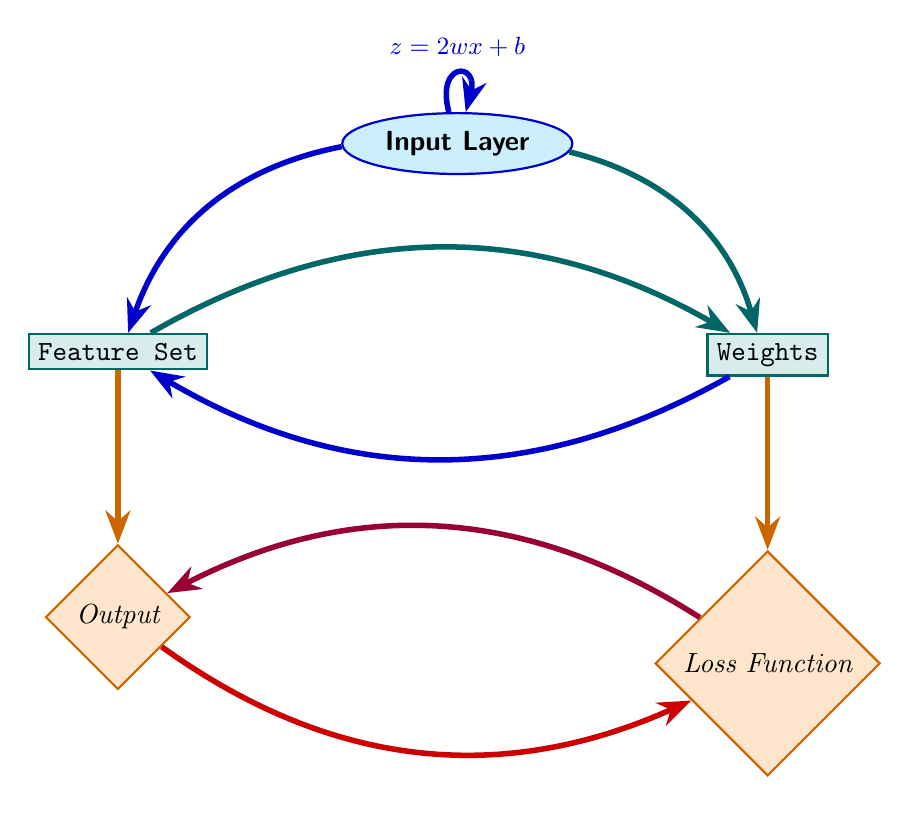
\begin{tikzpicture}[
    >=Stealth, 
    node distance=3cm, 
    thick, 
    process/.style={ellipse, draw=blue!80!black, fill=cyan!20, minimum width=4em, font=\sffamily\bfseries, text=black},
    data/.style={rectangle, draw=teal!80!black, fill=teal!15, minimum width=4em, font=\ttfamily, text=black},
    relation/.style={diamond, draw=orange!80!black, fill=orange!20, minimum width=3em, font=\itshape, text=black}
]

% Nodes
\node[process] (input)        {Input Layer};
\node[data, below left=of input]   (feature)     {Feature Set};
\node[data, below right=of input]  (weights)     {Weights};
\node[relation, below=2.2cm of feature] (output) {Output};
\node[relation, below=2.2cm of weights] (loss)   {Loss Function};

% Edges
\draw[->, teal!80!black, line width=2pt] (input) edge[bend left] (weights);
\draw[->, blue!80!black, line width=2pt] (input) edge[bend right] (feature);
\draw[->, orange!80!black, line width=2pt] (feature) -- (output);
\draw[->, orange!80!black, line width=2pt] (weights) -- (loss);
\draw[->, red!80!black, line width=2pt] (output) edge[bend right] (loss);
\draw[->, purple!80!black, line width=2pt] (loss) edge[bend right] (output);
\draw[->, teal!80!black, line width=2pt] (feature) edge[bend left=30] (weights);
\draw[->, blue!80!black, line width=2pt] (weights) edge[bend left=30] (feature);

% Self-loop
\draw[->, blue!80!black, line width=2pt] (input) edge[loop above, looseness=8] node[above, yshift=2pt, font=\small] {$z = 2wx + b$} (input);

\end{tikzpicture}
\end{document}